%% 
%% Copyright 2007-2019 Elsevier Ltd
%% 
%% This file is part of the 'Elsarticle Bundle'.
%% ---------------------------------------------
%% 
%% It may be distributed under the conditions of the LaTeX Project Public
%% License, either version 1.2 of this license or (at your option) any
%% later version.  The latest version of this license is in
%%    http://www.latex-project.org/lppl.txt
%% and version 1.2 or later is part of all distributions of LaTeX
%% version 1999/12/01 or later.
%% 
%% The list of all files belonging to the 'Elsarticle Bundle' is
%% given in the file `manifest.txt'.
%% 
%% Template article for Elsevier's document class `elsarticle'
%% with harvard style bibliographic references

% \documentclass[preprint,12pt,authoryear]{elsarticle}

%% Use the option review to obtain double line spacing
%% \documentclass[authoryear,preprint,review,12pt]{elsarticle}

%% Use the options 1p,twocolumn; 3p; 3p,twocolumn; 5p; or 5p,twocolumn
%% for a journal layout:
%% \documentclass[final,1p,times,authoryear]{elsarticle}
%% \documentclass[final,1p,times,twocolumn,authoryear]{elsarticle}
%% \documentclass[final,3p,times,authoryear]{elsarticle}
% \documentclass[final,3p,times,twocolumn,authoryear]{elsarticle}
%% \documentclass[final,5p,times,authoryear]{elsarticle}
%\documentclass[journal, a4paper]{IEEEtran}
\documentclass[final,5p,times,twocolumn,authoryear]{elsarticle}
\usepackage{graphicx}
\usepackage{threeparttable}
\usepackage{float}
\biboptions{comma,square,sort&compress}
\usepackage{url} %to format url
\def\UrlBreaks{\do\A\do\B\do\C\do\D\do\E\do\F\do\G\do\H\do\I\do\J
\do\K\do\L\do\M\do\N\do\O\do\P\do\Q\do\R\do\S\do\T\do\U\do\V
\do\W\do\X\do\Y\do\Z\do\[\do\\\do\]\do\^\do\_\do\`\do\a\do\b
\do\c\do\d\do\e\do\f\do\g\do\h\do\i\do\j\do\k\do\l\do\m\do\n
\do\o\do\p\do\q\do\r\do\s\do\t\do\u\do\v\do\w\do\x\do\y\do\z
\do\.\do\@\do\\\do\/\do\!\do\_\do\|\do\;\do\>\do\]\do\)\do\,
\do\?\do\'\do+\do\=\do\#} 
\usepackage{nomencl}
\setlength{\nomlabelwidth}{1.6cm}
\setlength{\nomitemsep}{-\parsep}
\makenomenclature
\usepackage{etoolbox}
\renewcommand\nomgroup[1]{%
  \item[\bfseries
  \ifstrequal{#1}{I}{Indices}{%
  \ifstrequal{#1}{P}{Parameters}{%
  \ifstrequal{#1}{V}{Variables}{}}}%
]}
% 
%% For including figures, graphicx.sty has been loaded in
%% elsarticle.cls. If you prefer to use the old commands
%% please give \usepackage{epsfig}

%% The amssymb package provides various useful mathematical symbols
\usepackage{amssymb}
\usepackage{amsmath}
%% The amsthm package provides extended theorem environments
%% \usepackage{amsthm}

%% The lineno packages adds line numbers. Start line numbering with
%% \begin{linenumbers}, end it with \end{linenumbers}. Or switch it on
%% for the whole article with \linenumbers.
%% \usepackage{lineno}

\journal{International Journal of Electrical Power & Energy Systems}


\begin{document}

\begin{frontmatter}

\title{Co-optimized Trading of Hybrid Wind Power Plant with Retired EV Batteries in Energy and Reserve Markets under Uncertainties}



\author[add1]{Sen Zhan} \ead{s181239@student.dtu.dk}
\author[add2]{Peng Hou\corref{cor1}} \ead{houpeng@shanghai-electric.com}
\author[add3]{Peter Enevoldsen} \ead{peter.enevoldsen@envisionenergy.dk}
\author[add1]{Guangya Yang} \ead{gyy@elektro.dtu.dk}
\author[add2]{Jiangsheng Zhu} \ead{zhujsh@shanghai-electric.com}
\author[add4]{Joshua Eichman} \ead{joshua.eichman@nrel.gov}
\author[add5]{Mark Z. Jacobson} \ead{jacobson@stanford.edu}

\address[add1]{Center of Electrical Engineering, Technical University of Denmark, Denmark}
\address[add2]{SEWPG European Innovation Center, Denmark}
\address[add3]{Centre for Energy Technologies, Aarhus University, Denmark}
\address[add4]{National Renewable Energy Laboratory, USA}
\address[add5]{Department of Civil and Environmental Engineering, Stanford University, USA}


\cortext[cor1]{Corresponding author at: SEWPG European Innovation Center, 8000 Aaruhus, Denmark}


\begin{abstract}
To be competitive in the electricity markets, various technologies have been reported to increase profits of wind farm owners. Combining battery storage system, wind farms can be operated as conventional power plants which promotes the integration of wind power into the power grid. However, high expenses on batteries keep investors away. Retired EV batteries, fortunately,  still have enough capacity to be reused and could be obtained at a low price. In this work, a two-stage optimization of a wind energy retired EV battery-storage system is proposed. The economic performance of the proposed system is examined concerning its participation in the frequency containment normal operation reserve (FCR-N) market and the spot market simultaneously. To account uncertainties in the wind farm output, various electricity market prices, and up/down regulation status, a scenario-based stochastic programming method is used. The sizing of the equipment is optimized on top of daily operations of the hybrid system which formulates a mixed-integer linear programming (MILP) problem. Scenarios are generated with the Monte Carlo simulation (MCS) and Roulette Wheel Mechanism (RWM), which are further reduced with the simultaneous backward method (SBM) to increase computational efficiency. A 21 MW wind farm is selected as a case study. The optimization results show that by integrating with a retired EV battery-storage system (RESS) and a bi-directional inverter, the wind farm can increase its profits significantly when forwarding bids in both of the aforementioned electricity markets.

\end{abstract}

\begin{keyword}
 retired EV battery-storage system (RESS) \sep FCR-N market \sep spot market \sep  MILP

\end{keyword}

\end{frontmatter}

\nomenclature[I]{$t$}{Hour index from 1 - 24 in a day}
\nomenclature[I]{$d$}{Day index from 1 - 365 in a year}
\nomenclature[I]{$\omega$}{Scenario index}
\nomenclature[I]{$i$}{Uncertain parameter index}
\nomenclature[I]{$j$}{Interval index}
\nomenclature[V]{$\pi$}{Scenario probability}
\nomenclature[V]{$Z$}{Binary variables indicating options being chosen}
\nomenclature[V]{$\epsilon$}{Random numbers generated in the simulation}
\nomenclature[P]{$EP$}{Spot market price}
\nomenclature[P]{$P^{wt}$}{Power generation}
\nomenclature[P]{$SoH$}{The ratio between the usable capacity of degraded battery and the nominal capacity}
\nomenclature[V]{$P^{spot,wt}$}{The power traded in spot market generated from wind farm }
\nomenclature[V]{$P^{dis}$}{The power discharged from RESS }
\nomenclature[V]{$P^{ch}$}{The charging power for RESS }
\nomenclature[V]{$R$}{The bidden capacity for upward regulation  }
\nomenclature[P]{$FCRN$}{The FCR-N market price}
\nomenclature[V]{$P^{ch,wt}$}{The power that is used for charging RESS from wind farm }
\nomenclature[V]{$P^{ch,up}$}{Potential electricity inflow into RESS from upward regulation}
\nomenclature[P]{$T$}{Scenario span, 24 hours}
\nomenclature[P]{$E^{EVB}$}{Brand new battery capacity}
\nomenclature[P]{$\alpha$}{The ratio between the retired EV battery price and the brand new battery price}
\nomenclature[V]{$E^{charge}$}{Absolute charge content of the RESS}
\nomenclature[P]{$\eta^{ch}$,$\eta^{dis}$}{RESS charge/discharge efficiency}
\nomenclature[P]{$\eta^{inv}$}{Inverter efficiency for both directions}
\nomenclature[P]{$\eta^{up}$,$\eta^{down}$}{Percentages of activated power to bidden capacity for upward/downward regulation}
\nomenclature[P]{$M$}{Arbitrarily big number in big M method}
\nomenclature[V]{$E^{RESS}$}{RESS capacity}
\nomenclature[P]{$\delta^{up}$,$\delta^{down}$}{Binary numbers used to indicate upward/downward regulation }
\nomenclature[V]{$SoC$}{State of charge}
\nomenclature[V]{$N$}{Optimized battery number of RESS}
\nomenclature[V]{$P^{spot}$}{Bidden electricity in spot market}
\nomenclature[V]{$P^{inv}$}{The bi-directional inverter power}
\nomenclature[P]{$RPP^{up}$}{Upward regulating power price }
\nomenclature[P]{$RPP^{down}$}{Downward regulating power price }
\nomenclature[P]{$\lambda^{inv}$}{Inverter price }
\nomenclature[P]{$\lambda^{EVB}$}{Brand new EV battery price }
\nomenclature[V]{$P^{ch,down}$}{Potential electricity inflow into RESS from downward regulation  }
\nomenclature[V]{$P^{acti,up}$}{Potential electricity inflow into FCR-N market from upward regulation }
\nomenclature[V]{$\delta^{ch}$,$\delta^{dis}$}{Binary variables indicating charging/discharging state of RESS }
\nomenclature[V]{$\delta^{1}$,$\delta^{2}$}{Binary variables indicating if bid is made to FCR-N market}
\nomenclature[P]{$\delta^{3}$}{Binary numbers indicating if power generation is over 0.3 MW }
\nomenclature[P]{$\delta^{4}$}{Binary numbers indicating if FCR-N market price is over 80\% of spot market price}
\nomenclature[P]{$\delta^{5}$}{Binary numbers indicating if spot market price is non-positive}
\printnomenclature


%\linenumbers

%% main text
\section{Introduction}
\label{sec:introduction}

Electrical Vehicles (EVs) have been scoped as the transition transportation technology to replace internal combustion engine vehicles (ICEVs) \cite{Kester2018PromotingDiffusion, Ajanovic2018ElectricProblem}, however, despite academic consensus, the deployment of EVs remains low with a representation of, less than 1\% of the combined global vehicle fleet \cite{InternationalEnergyAgencyIEA2017GlobalCounting}. Multiple reasons for the slow transition have been examined ranging from battery performance \cite{Ajanovic2018ElectricProblem}, vehicle costs \cite{Sovacool2017TheAgenda}, range limitations \cite{Noel2019FearAnxiety}, etc., and are frightening similar as determined a decade ago \cite{Sovacool2009BeyondTransition}. Simultaneously, advocates for EVs have been using the arguments of vehicle-to-grid (V2G), which enables strategic storing and exchange of electricity \cite{Sovacool2017TheAgenda}. However, few, if any studies have adequately examined the potential usage of EVs and EV batteries after the expired lifetime in combination with multi-megawatt wind turbines. Instead recent studies have focused on the combination of PV and retired EV batteries, and found that a) residual capacities can be exploited \cite{HUANG201980}, b) power management and selection strategies are required to optimize the value of the retired battery \cite{8279474}, and c) the environmental, social and economic profiles of EV batteries are improved due to a minimization of the recycling rate \cite{TANG20194304}. Assuming the same consequences for retired EV batteries, it 
would inevitably increase the value of lifetime EVs, and potentially add to the policy mechanisms, which especially seems to be lacking in Denmark \cite{Kester2018PromotingDiffusion}. As a matter of fact, only  8,746 EVs (plug-in hybrids and all-electric vehicles) were registered in Denmark by the end of 2017 \cite{Bilimp}, which is far less than the Scandinavian neighbours Norway (209,122)  \cite{Elbil} and Sweden (50,304) \cite{BilSweden}. This being despite the fact that Denmark has excellent wind resources \cite{Enevoldsen2016OnshoreRisks},  a high penetration of wind power in its electricity mix (44\% of the demand in 2017) \cite{Pineda2018}, and several days with a surplus of electricity and thereby negative electricity prices \cite{Hou2017OptimizingDenmark}.

Using batteries for electrical storage system (ESS) is not a novel thought, and especially lithium-ion battery was brought up in several studies as a prominent technology for load shifting and peak shaving demands \cite{Luo2015OverviewOperation, Zakeri2015Corrigendum569596,Wen2018Multi-time-scaleStorage, Fang2018DynamicSystems}, and highlighted for its capabilities of low standby losses and high energy efficiencies (60 - 95\%) \cite{Chen2009ProgressReview}. Using batteries to increases the profitability of wind farms have also been proposed before \cite{Hou2018CooperationMarkets}, as several studies demonstrated methods for lucrative bidding strategies on the day-ahead markets when combining batteries and wind farms \cite{Baringo2016OfferingApproach, Dai2015OptimalMarket}. Furthermore, applying batteries as the cornerstone technology in ESS was concluded to be the most profitable approach to provide primary frequency service in the Danish reserve electricity market almost a decade ago \cite{Jozef2011AalborgA}.

This study will investigate solutions to a) The fluctuations in Danish electricity prices due to the heavy reliance on wind power, and b) The investment opportunities of installing retired EV batteries in Danish operational offshore wind farms. 

\begin{figure*}
\centering
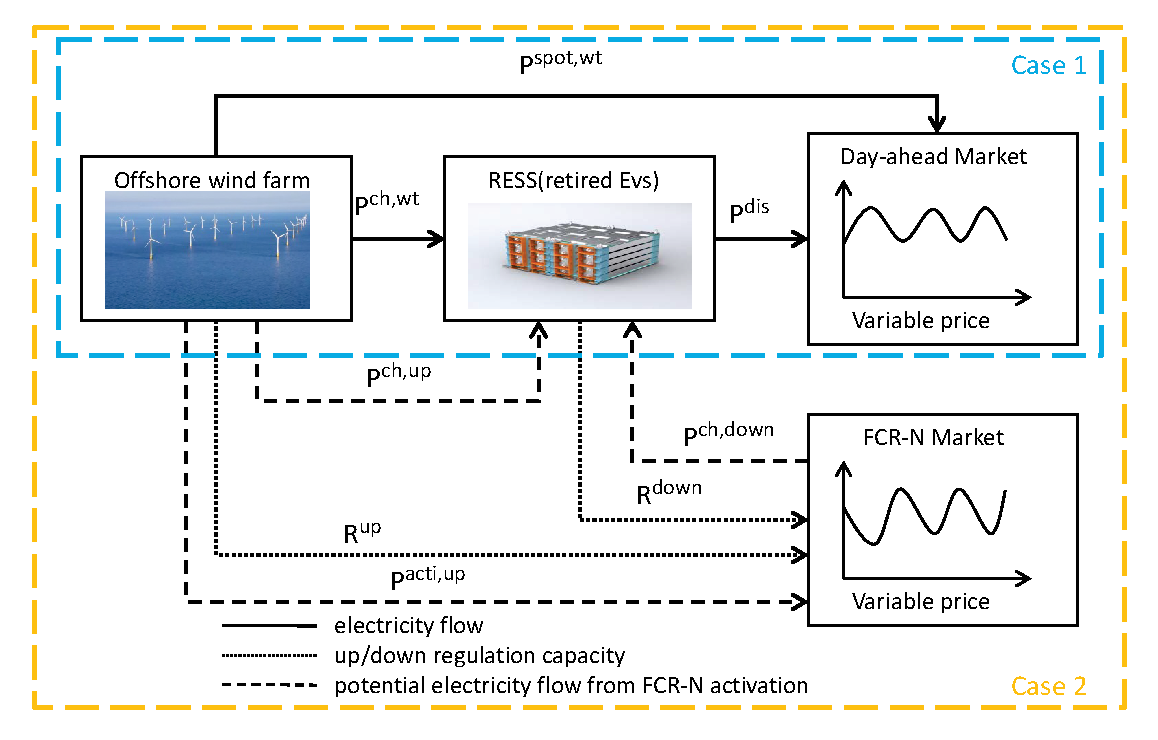
\includegraphics[width = 0.8\textwidth]{figures/model.eps}
\caption{Hybrid wind farm-RESS system schematic layout}
\label{fig:model}
\end{figure*}

In order to examine such challenges, the hybrid wind farm - retired EV batteries system is expected to participate in both the day-ahead and the FCR-N market. As a comparison, another case in which the wind farm only participates in the spot market is also studied, both shown in Fig. \ref{fig:model}. According to the rule of Danish transmission system operating, the balance responsible parties (BRPs, referring to the hybrid system in this study) merely need to provide a small amount of energy to mitigate the frequency deviation and get remunerated mainly by the bidden power capacity. Therefore, the electricity generated from the wind turbines can be sold at the spot market or caters for upward regulations of the FCR-N market, with part energy or the surplus going into the RESS or possibly both.

Since discharging the battery will incur high cost and reduce the battery lifetime and performance
obviously, the RESS works as downward regulation medium and receives electricity from the FCR-N market when downward regulation is needed. The upward regulation in the FCR-N market can be handled by controlling the wind turbines in the de-rated mode and releasing those when needed. 

The research materials and methods are based upon the examination of the potential profitability of integrating retired EV batteries in a Danish operational offshore wind farm. Furthermore, web searches have been conducted to inform about statistics of EVs and the market prices in Denmark. The following sections describes the methodology and materials applied for the core elements of this research. 
\section{Problem Formulation}
In this work, a scenario-based stochastic programming method is employed to cope with the inherent uncertainties of the optimization problem, including the power generation, the spot market prices, the FCR-N market prices, the regulating market (upward and downward) prices and the FCR-N service activation states. The framework has been examined in \cite{Niknam2012AnOperation, Bornapour2019} and concluded to be an efficient and  effective method to account uncertainties for scheduling problems. To convexify the problem, the big M method is adopted to linearize the bi-linear term. The scenario generation and reduction are specified at the beginning of this part while the mathematical model of the optimization problem is given in the end.
\subsection{Scenario generation}
The uncertain parameters listed in the previous paragraph are determined with generated scenarios by Monte Carlo Simulation (MCS) and Roulette Wheel Mechanism (RWM). Although other methods such as rejection method \cite{lectureNote} and alias method \cite{lectureNote} can be used to generate random variables with discrete distribution, RWM is simpler and does not require complex set-up procedure. Indeed, RWM has been applied in \cite{Niknam2012AnOperation, Bornapour2019, Ahmadi2016}. Numerical results show the capability of this method \cite{Ahmadi2016}. The realization process is summarized as follows.

\begin{figure}[h]
    \centering
    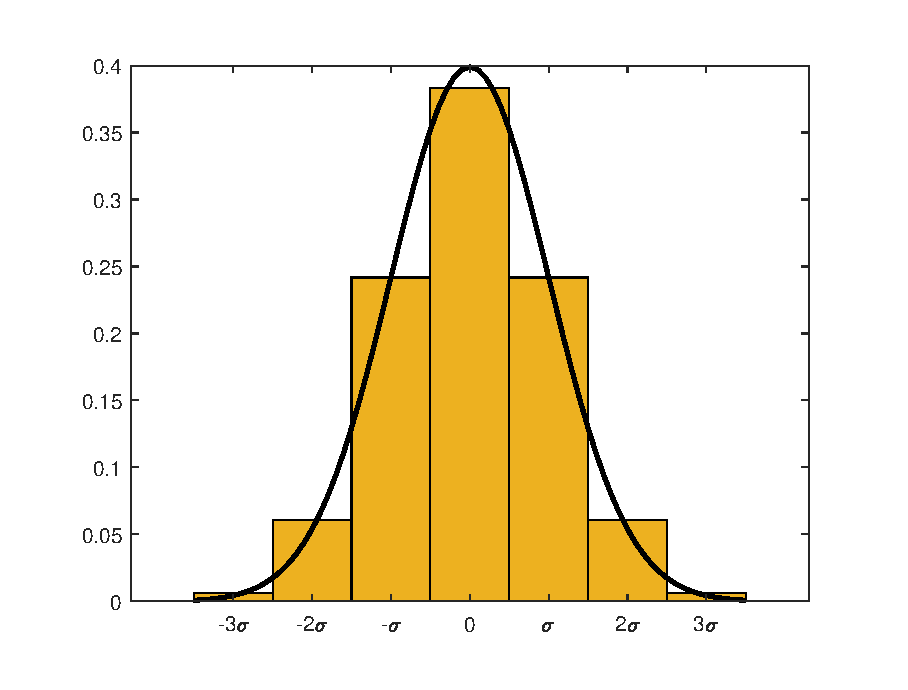
\includegraphics[width=0.5\textwidth,height =0.25\textwidth]{figures/distribution.eps}
    \caption{Discretization of forecast errors distribution}
    \label{fig:distribution}
\end{figure}

The Probability Distribution Function (PDF) is used to generate a set of possible options and corresponding probabilities based on forecast errors of the power generation and the different market prices, while for the FCR-N service activation states, the historical frequency is assumed as the probability for each possible state. As shown in Fig. \ref{fig:distribution}, discretization and normalization are performed on the continuous probability distribution, generating 7 segments with an interval of standard deviation ($\sigma$) \cite{Niknam2012AnOperation}. The probability distribution of reserve service activation states is shown in Fig. \ref{fig:reserve}. To be more specific, the prediction error of the wind power can be obtained from \cite{Hodge2012}. In our case, its $\sigma$ is taken as 5\% for Denmark. From \cite{Karabiber2019, Cerjan2019}, a $\sigma$ of 10\% is a reasonable estimation of the prediction error for day-ahead market price. The prediction errors are also assumed as 10\% for the FCR-N market and regulating market price.

\begin{figure}[h]
    \centering
    \includegraphics[width=0.5\textwidth,height =0.25\textwidth]{figures/reserve.eps}
    \caption{Reserve service activation state probability distribution }
    \label{fig:reserve}
\end{figure}

\begin{figure}[h]
    \centering
    \includegraphics[width=0.5\textwidth]{figures/MCS.eps}
    \caption{Accumulated probability distribution.(1):Power generation, FCR-N market prices, spot market prices and regulating market prices. (2): Reserve service activation states.}
    \label{fig:mcs}
\end{figure}
Afterwards, random numbers ($\epsilon_t^{wt}$, $\epsilon_t^{FCR-N}$, $\epsilon_t^{spot}$, $\epsilon_t^{up}$,
$\epsilon_t^{down}$,
$\epsilon_t^R$) ranging from [0,1] are generated for each hour. As in Fig. \ref{fig:mcs}, the intervals where the random numbers fall in are taken as the corresponding options for each uncertain parameter. A scenario is therefore defined as a set of random numbers for each hour within a day:
\begin{equation} \label{eq:scenario}
\begin{split}
 \omega= \{\epsilon_1^{wt}, \epsilon_1^{FCR-N}, \epsilon_1^{spot},\epsilon_1^{up},\epsilon_1^{down}, \epsilon_1^R,\epsilon_2^{wt}, \epsilon_2^{FCR-N},\epsilon_2^{spot},\epsilon_2^{up},\\ \epsilon_2^{down}, \epsilon_2^R,\cdots,\epsilon_T^{wt}, \epsilon_T^{FCR-N}, \epsilon_T^{spot}, \epsilon_T^{up},\epsilon_T^{down},\epsilon_T^R \}
\end{split}
\end{equation}

A typical scenario is shown in Fig. \ref{fig:scenario}, where the uncertain parameters in a day are all determined with certain values. For example, in the first hour, the power is no more uncertain parameter, but fixed at just below 15 MWh. With all the scenarios, the stochastic programming problem is transformed into its deterministic equivalent. It can also be observed that the spot market prices intersect with the FCR-N market prices indicating profitability of biding in the FCR-N market.

In order to obtain the probability of each scenario, $Z_{\omega,t,i,j}$ is introduced to indicate the MCS results where i is the uncertain parameter index and j is the interval index. The rule is that originally $Z_{\omega,t,i,j}$ are all set as 0. When the corresponding interval is taken in the simulation, the related $Z_{\omega,t,i,j}$ is changed into 1. Suppose $\pi_{i,j}$ is the probability of the corresponding interval being taken, which is neither time nor scenario dependent, the normalized probability \cite{Niknam2012AnOperation} of scenario $\omega$ is then:
\begin{equation} \label{eq:scenarioProbability}
\pi_{\omega} = \frac{\prod_{t=1}^T \prod_{i=1}^I\sum_{j=1}^J(Z_{\omega,t,i,j}\pi_{i,j})}{\sum_{\omega}^{\Omega}\prod_{t=1}^T \prod_{i=1}^I\sum_{j=1}^J(Z_{\omega,t,i,j}\pi_{i,j})}
\end{equation}
\subsection{Scenario reduction}
Large number of scenarios usually indicate better approximation of the original problem, but also with longer computation time and larger complexity. In this research, the simultaneous backward method (SBM) which concurrently considers scenario distance and scenario probability is employed. Numerical tests have shown that SBM provides accurate solutions to the optimal reduction problem \cite{1304379} and is also used in researches such as \cite{Niknam2012AnOperation}. The principle of scenario reduction is to reduce the scenario amount by deleting scenarios with lower probability and bundling similar scenarios, while keeping the characteristics as much as possible. The SBM is described as follows:
\begin{enumerate}
    \item Consider $\Omega$ as the initial scenario set. The distance matrix $DT$ is defined where $\omega, \omega' \in  \Omega$:
    \begin{equation} \label{eq:scenarioDistance}
DT_{\omega,\omega'}  = \left\{
\begin{array}{ll}
\sqrt{ \sum_{t =1, i = 1, j = 1}^{T,I,J}(Z_{\omega,t,i,j}-Z_{\omega',t,i,j})^2} &{ \omega \neq \omega'}\\
 Inf & {\omega = \omega'}
\end{array} \right.
    \end{equation}
    \item Define probability-distance matrix $PD$ as :
    \begin{equation}
    PD_{\omega,\omega'} = \pi_\omega DT_{\omega,\omega'}    
    \end{equation}
    \item   Select $d, r$ where $PD_{d,r}$ is the smallest entry in the matrix $PD$. Delete scenario d in scenario set $\Omega$, $\pi_r = \pi_r + \pi_d$.
    \item Delete the row d and column d in distance matrix DT.
    \item Repeat the steps 2-4 until the required scenario amount is obtained.
\end{enumerate}

\begin{figure}
    \centering
    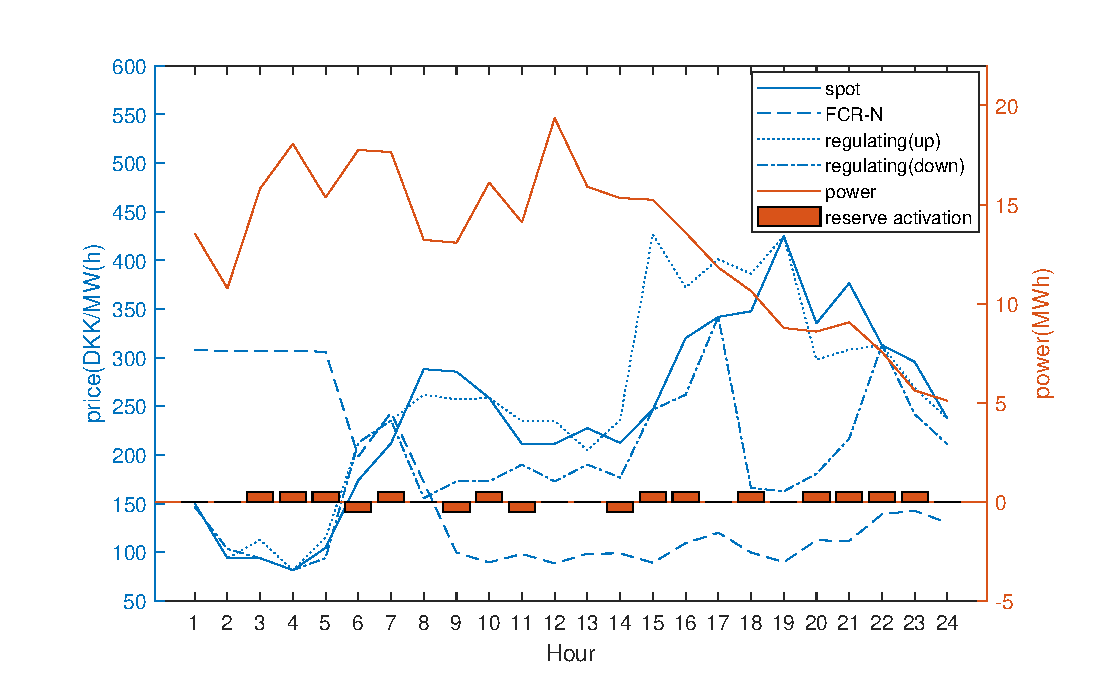
\includegraphics[width=0.5\textwidth]{figures/scenario.eps}
    \caption{A typical scenario for 2nd November, 2017 with 1 indicating upward regulation, -1 being downward and 0 being reserve services not activated.}
    \label{fig:scenario}
\end{figure}

\subsection{Mathematical model}

In order to verify the financial benefit of integrating the RESS and participating the FCR-N market, three cases are studied. In the base case, the wind farm without the storage system participates the spot market only and bids all the predicted power generation into the spot market, the revenue of which for a whole year is as Eq. (\ref{eq:revenue1}). In case 1, the wind farm purchases RESS and participates the spot market, while bids are made in both the spot market and the FCR-N market in case 2.
\begin{equation} \label{eq:revenue1}
R^{base} =\sum_{d}^D \sum_{\omega =1}^{\Omega}\pi_{\omega,d}\sum_{t = 1}^T \left\{EP_{t,\omega,d}P_{t,\omega,d}^{wt}1 \right\}
\end{equation}
\subsubsection{Case 1}
After the RESS is introduced into the system, the wind farm can perform arbitrage in the spot market. The yearly revenue is:
\begin{equation} \label{eq:revenue2}
\begin{split}
R^{case1} =\sum_{d}^D \sum_{\omega =1}^{\Omega}\pi_{\omega,d}\sum_{t = 1}^T \{ EP_{t,\omega,d}P_{t,\omega,d}^{spot}1  \}
\end{split}
\end{equation}

The benefit is considered as revenue difference before and after RESS introduction. The economic analysis is performed with 20 year's period since this is the wind turbine's lifetime. The net present value (NPV) of benefit is:
\begin{equation} \label{eq:benefit}
\text{NPV-B}^1 =\text{NPV-R}^1 - \text{NPV-R}^b = \sum_{y = 1}^{20} \frac {R^{case1} - R^{base}} {(1+d_r)^{y-1}}
\end{equation}
where the superscript b and 1, 2 (in following section) stand for the base case, case 1 and case 2 respectively. 

The cost is considered as three parts: the initial investment of the RESS and the bi-directional inverter, the replacement cost (the cost of replacing the RESS and inverter with new one at the end of their lifetime), and the operation and maintenance cost (1\% of investment each year for both) \cite{Zhang2017ComparativeOperation}. In case 1 and 2, two scenarios are considered concerning the price of retired battery, which is 15\% of the brand new EV battery price in the optimistic scenario and 30\% in the pessimistic scenario. The NPV of the cost is therefore:
\begin{equation} \label{eq:cost}
\begin{split}
 \text{NPV-C} = P^{inv}\lambda^{inv}[1+\frac{1}{(1+d_r)^{10}}+ \sum_{y =1}^{20} \frac{r_{O\&M}}{(1+d_r)^{y-1}}]\\
 +\alpha_i N E^{EVB} \lambda^{EVB} [1+\frac{1}{(1+d_r)^{7}}+\frac{1}{(1+d_r)^{14}} + \sum_{y =1}^{20}\frac{r_{O\&M}}{(1+d_r)^{y-1}}]  
\end{split}
\end{equation}
where the inverter is assumed to be replaced after 10 year's operation, while the replacement for the RESS is done each 7 years, as specified in Table \ref{tab:cba}.\\

\noindent
\textbf{Obj.}
\begin{equation} \label{eq:outerobj}
\text{Max.} \quad \text{NPV-P} =  \text{NPV-B}^1 -\text{NPV-C} 
\end{equation}
\noindent
\textbf{S.t.}
\begin{equation} \label{eq:inverter}
P^{inv} \geq 0   
\end{equation}
\begin{equation} \label{eq:capacity}
E^{cap}  = N E^{EVB}   \text{SoH}, N \geq 0
\end{equation}
\begin{equation} \label{eq:spot}
P_{t,\omega,d}^{spot} = P_{t,\omega,d}^{spot,wt} +P_{t,\omega,d}^{dis}, \forall t,\forall \omega,\forall d
\end{equation}
\begin{equation} \label{eq:windfarmequilibrium1}
P_{t,\omega,d}^{ch,wt} + P_{t,\omega,d}^{spot,wt} = P_{t,\omega,d}^{wt},\forall t,\forall \omega,\forall d
\end{equation}
\begin{equation} \label{eq:charge}
P_{t,\omega,d}^{ch} = P_{t,\omega,d}^{ch,wt},\forall t,\forall \omega,\forall d
\end{equation}
\begin{equation} \label{eq:SoCequi}
E^{charge}_{t+1,\omega,d} = E^{charge}_{t,\omega,d}+(\eta^{ch} \eta^{inv} P_{t,\omega,d}^{ch}-\frac{P_{t,\omega,d}^{dis}}{\eta^{dis} \eta^{inv}})1,\forall t,\forall \omega,\forall d
\end{equation}
\begin{equation} \label{eq:SoClimit}
SoC_{min}E^{cap}\leq E^{charge}_{t,\omega,d} \leq SoC_{max}E^{cap},\forall t,\forall \omega,\forall d
\end{equation}
\begin{equation} \label{eq:SoCinitial}
E^{charge}_{1,\omega,d} = E^{charge}_{T + 1,\omega,d} = E^{charge}_{initial},\forall \omega,\forall d
\end{equation}
\begin{equation} \label{eq:spotlimit}
0 \leq P_{t,\omega,d}^{spot,wt} \leq P_{t,\omega,d}^{wt},\forall t,\forall \omega,\forall d 
\end{equation}
\begin{equation} \label{eq:windcharge}
0 \leq P_{t,\omega,d}^{ch,wt} \leq P_{t,\omega,d}^{wt} ,\forall t,\forall \omega,\forall d 
\end{equation}
\begin{equation} \label{eq:inv+}
0 \leq P_{t,\omega,d}^{ch} \leq P^{inv} ,\forall t,\forall \omega,\forall d 
\end{equation}
\begin{equation} \label{eq:inv-}
0 \leq P_{t,\omega,d}^{dis} \leq P^{inv},\forall t,\forall \omega,\forall d  
\end{equation}
\begin{equation} \label{eq:combinational}
P_{t,\omega,d}^{ch} P_{t,\omega,d}^{dis}  = 0, \forall t,\forall \omega,\forall d  
\end{equation}

The objective function is the minus NPV of profit of the wind farm owner. In (\ref{eq:inverter}) and  (\ref{eq:capacity}), the capacity of inverter and RESS are constrained as continuous and discrete variables respectively. (\ref{eq:spot}) states the bidden electricity in the spot market while  (\ref{eq:windfarmequilibrium1}) shows the electricity balance of the wind farm. (\ref{eq:charge}) indicates that wind power is the only charging source. The SoC balance, and upper/lower limits of SoC are shown in  (\ref{eq:SoCequi}) - (\ref{eq:SoClimit}). To guarantee the energy will be used out at the end of each day, (\ref{eq:SoCinitial}) is applied as boundary conditions. (\ref{eq:spotlimit}) and (\ref{eq:windcharge}) ensures the energy that flows into the spot market or the RESS is less than the generated energy. In (\ref{eq:inv+}) and (\ref{eq:inv-}), the constraints from inverter size are applied. By nature, the RESS cannot be charged and discharged simultaneously, which is stated in (\ref{eq:combinational}) as a combinational constraint.

Binary pair of variables, $\delta_{t,\omega,d}^{ch}$ / $\delta_{t,\omega,d}^{dis}$ are introduced to help linearize (\ref{eq:combinational}), which represent the charging/discharging state of the RESS. The big M method is implemented in this work to linearize the bi-linear term, where $M_1$ and $M_2$ in later paragragh are arbitrarily big number, which substitutes (\ref{eq:combinational}) with:
\begin{equation} \label{eq:binary}
\delta_{t,\omega,d}^{ch},\delta_{t,\omega,d}^{dis} \in \{0,1\}, \delta_{t,\omega,d}^{ch}+\delta_{t,\omega,d}^{dis} \leq 1, \forall t,\forall \omega,\forall d
\end{equation}
\begin{equation} \label{eq:bigM3}
0 \leq  P_{t,\omega,d}^{ch} \leq M_1 \delta_{t,\omega,d}^{ch}, \forall t,\forall \omega,\forall d
\end{equation}
\begin{equation} \label{eq:bigM4}
0 \leq  P_{t,\omega,d}^{dis} \leq M_1\delta_{t,\omega,d}^{dis}, \forall t,\forall \omega,\forall d
\end{equation}
\subsubsection{Case 2}
In case 2, the yearly revenue for the wind farm owner comprises the revenue from the day-ahead electricity market, from the bidden capacity in the FCR-N market and from the FCR-N service activation energy which is settled per MWh with the regulating power prices (RPP) \cite{symmetrical}. For the FCR-N market, the Danish TSO Energinet requires simultaneous and symmetrical upward and downward regulation reserve bid \cite{symmetrical}. Therefore, the upward bids and downwards bids can be described with one term $R_{t,\omega,d}$. 
\begin{equation} \label{eq:revenue3}
\begin{split}
R^{case2} =\sum_{d}^D \sum_{\omega =1}^{\Omega}\pi_{\omega,d}\sum_{t = 1}^T \{ EP_{t,\omega,d}P_{t,\omega,d}^{spot}1 + R_{t,\omega,d}FCRN_{t,\omega,d} \\+ P_{t,\omega,d}^{acti,up}RPP_{t,\omega,d}^{up}1 - P_{t,\omega,d}^{ch,down}RPP_{t,\omega,d}^{down}1 \}
\end{split}
\end{equation}

\noindent
\textbf{Obj.}
\begin{equation} \label{eq:outerobj2}
\text{Max.} \quad \text{NPV-P} = \text{NPV-B}^2 - \text{NPV-C}
\end{equation}
\noindent
\textbf{S.t.}
$$(\ref{eq:inverter}) - (\ref{eq:spot})$$
\begin{equation} \label{eq:windfarmequilibrium}
P_{t,\omega,d}^{ch,wt} + P_{t,\omega,d}^{spot,wt} = P_{t,\omega,d}^{wt}-R_{t,\omega,d} ,\forall t,\forall \omega,\forall d
\end{equation}
\begin{equation} \label{eq:charge2}
P_{t,\omega,d}^{ch} = P_{t,\omega,d}^{ch,wt
}+  P_{t,\omega,d}^{ch,up} + P_{t,\omega,d}^{ch,down},\forall t,\forall \omega,\forall d
\end{equation}
$$(\ref{eq:SoCequi}) - (\ref{eq:SoCinitial})$$
\begin{equation} \label{eq:upregulation}
P_{t,\omega,d}^{acti,up}= \eta^{up}
\delta_{t,\omega,d}^{up}  R_{t,\omega,d} ,\forall t,\forall \omega,\forall d
\end{equation}
\begin{equation} \label{eq:upactivation}
0 \leq P_{t,\omega,d}^{ch,up} \leq (1-\eta^{up}) \delta_{t,\omega,d}^{up} R_{t,\omega,d} ,\forall t,\forall \omega,\forall d
\end{equation}
\begin{equation} \label{eq:downregulation}
P_{t,\omega,d}^{ch,down} = \eta^{down} \delta_{t,\omega,d}^{down}   R_{t,\omega,d},\forall t,\forall \omega,\forall d 
\end{equation}
\begin{equation} \label{minbid}
  R_{t,\omega,d}\geq 0.3 \vee  R_{t,\omega,d} = 0,\forall t,\forall \omega,\forall d 
\end{equation}
\begin{equation} \label{eq:uplimit}
R_{t,\omega,d} \leq P_{t,\omega,d}^{wt}, \forall t,\forall \omega,\forall d 
\end{equation}
\begin{equation} \label{eq:downlimit}
R_{t,\omega,d}1 \leq  min\{ SoC_{max}E^{cap}-E^{charge}_{t,\omega,d},P^{inv}1 \},\forall t,\forall \omega,\forall d 
\end{equation}
$$(\ref{eq:spotlimit}) - (\ref{eq:inv-}),(\ref{eq:binary}) - (\ref{eq:bigM4}) $$

The objective function is the net present value of profit, where the NPV-C can be calculated as (\ref{eq:cost}), and $R_{case1}$ has to be replaced as $R_{case2}$ for the NPV-B in Eq. (\ref{eq:benefit}).  (\ref{eq:windfarmequilibrium}) sets the new electricity balance of the wind farm considering the reserved capacity for upward regulation. The charging power is stated as  (\ref{eq:charge2}) where $P_{t,\omega,d}^{ch,up}$ and  $P_{t,\omega,d}^{ch,down}$ denoting the potential inflow of electricity from the activated wind turbines if upward regulation is needed and from activated RESS if downward regulation is needed, respectively.  (\ref{eq:upregulation}) - (\ref{eq:downregulation}) defines aforementioned  $P_{t,\omega,d}^{acti,up}$,$P_{t,\omega,d}^{ch,up}$ and $P_{t,\omega,d}^{ch,down}$, where, $\delta_{t,\omega,d}^{up}$ and $\delta_{t,\omega,d}^{down}$ are a set of known binary numbers indicating if the TSO requires upward/downward regulations, and $\eta^{up}$ and $\eta^{down}$, both assumed to be 10\%, are the percentages of electricity flowing into or receiving from the FCR-N market since the capacity is what the FCR-N market really needs to maintain the frequency stability. When secondary frequency reserves (aFRR) are activated, the TSO releases the FCR-N reserve services, which happens 150 seconds \cite{symmetrical} after the frequency deviation, and the wind farm owner can collect the rest electricity generated from the wind turbines with the RESS. The minimum bidden FCR-N capacity is 0.3MW \cite{symmetrical}, which is constrained as (\ref{minbid}). Hourly bidden upward and downward regulation capacities are constrained as (\ref{eq:uplimit}) and (\ref{eq:downlimit}) respectively. The constraints (\ref{eq:inverter}) - (\ref{eq:spot}), (\ref{eq:SoCequi}) - (\ref{eq:SoCinitial}), (\ref{eq:spotlimit}) - (\ref{eq:inv-}) and (\ref{eq:binary}) - (\ref{eq:bigM4}) still apply to case 2.

Likewise, the big M method with binary variables $\delta_{t,\omega,d}^{1}$ / $\delta_{t,\omega,d}^{2}$ indicating whether is forwarded to the FCR-N market is performed on constraint (\ref{minbid}). Then, it can be rewritten as:
\begin{equation} \label{eq:binary2}
\delta_{t,\omega,d}^{1},\delta_{t,\omega,d}^{2} \in \{0,1\}, \delta_{t,\omega,d}^{1}+\delta_{t,\omega,d}^{2} = 1, \forall t,\forall \omega,\forall d
\end{equation}
\begin{equation} \label{eq:bigM1}
-M_2(1-\delta_{t,\omega,d}^{1}) \leq R_{t,\omega,d}\leq M_2(1-\delta_{t,\omega,d}^{1}), \forall t,\forall \omega,\forall d
\end{equation}
\begin{equation} \label{eq:bigM2}
-M_2(1-\delta_{t,\omega,d}^{2}) + 0.3 \leq R_{t,\omega,d}, \forall t,\forall \omega,\forall d
\end{equation}

The aforementioned model can be implemented by the wind farm owner for daily operations with a much shorter optimization span. However, for the strategy maker who needs to include the equipment sizes as the optimization variables and usually performs the optimization with a year's span (with constraint (\ref{eq:SoCinitial}) as daily boundary conditions), such binary variables  with high dimensionality in the model will severely undermine the computation efficiency and can even cause the model untractable with existing commercial solvers. In order to enhance the implementation performance of the large-scale MILP problem, following assumptions concerning the wind farm owner's behaviours are made to avoid the binary variables in the model: a) Always and only forward bids in the FCR-N market when power generation is over 0.3 MW and the predicted FCR-N market price is higher than 80\% of spot market price and b) Never bids RESS-stored electricity in the spot market if predicted price is non-positive.

The first assumption is made with respect to the minimum bids requirement in the FCR-N market and taking into account the potential electricity inflow and revenue from the reserve service activation. Afterwards, constraint (\ref{minbid}) can be transformed as:
\begin{equation} \label{eq:delta34}
\left\{
\begin{array}{lcl}
  R_{t,\omega,d} \geq 0.3 & & {\delta_{t,\omega,d}^3 \delta_{t,\omega,d}^4 = 1}\\
  R_{t,\omega,d} = 0 & & {\delta_{t,\omega,d}^3\delta_{t,\omega,d}^4 =  0}
\end{array} \right. , \forall t,\forall \omega,\forall d
\end{equation}
with $\delta_{t,\omega,d}^{3}$ indicating if the power generation is over 0.3 MW, $\delta_{t,\omega,d}^{4}$  indicating if the FCR-N market price is over 80\% of the spot market price. 

Simultaneous charging and discharging will incur electricity waste due to  inefficiency, which definitely results in revenue loss when the spot market price is positive \cite{Hou2018CooperationMarkets}.  Therefore, the constraint (\ref{eq:combinational}) can be decoupled naturally with the above assumptions. As a result, the constraints (\ref{eq:binary}) - (\ref{eq:bigM4}) can be replaced with:
\begin{equation} \label{eq:delta5}
P_{t,\omega,d}^{dis} \leq M_3\{[1- \delta_{t,\omega,d}^{3} \delta_{t,\omega,d}^{4}(\delta_{t,\omega,d}^{up} + \delta_{t,\omega,d}^{down})]  \vee (1- \delta_{t,\omga,d}^{5})\}, \forall t,\forall \omega,\forall d
\end{equation}
 where $\delta_{t,\omega,d}^{5}$ will be zero if the spot market price is non-positive. In essence, the constraint (\ref{eq:delta5}) limits that the RESS cannot discharge if the spot market price is non-positive or if the reserve services are activated. 
\subsection{Assumptions}
Apart form the assumptions made above, some other assumptions are made in the follows.

a) The predicted values for the power generation, the spot market prices, the FCR-N market prices, the regulating market prices, and the reserve activation states are assumed to be based on historical data for scenario generation.

b) The wind farm is assumed to be able to make predictions before the market closure, which is usually a day before real-time transaction.

c) The bids in the spot market and the FCR-N market are both assumed to be fully accepted.

d) To account for the impacts on performance of retired EV battery, the capacity, and the maximum and minimum charging/discharging is limited to short range in this work. The retired batteries are not designed to perform market arbitrage either, which means electricity from the day-ahead market is not used to charge the RESS.


\section{Case Study}
    In this part, several cases are studied to demonstrate the proposed method. The FCR-N market prices are from Energinet \cite{FCRNprice} while the spot market and regulating market prices are from Nordpool \cite{Nordpool}. The mathematical model is solved with CPLEX \cite{Cplex} based on YALMIP \cite{yalmip} toolbox on MATLAB.

\begin{figure}[h]
    \centering
    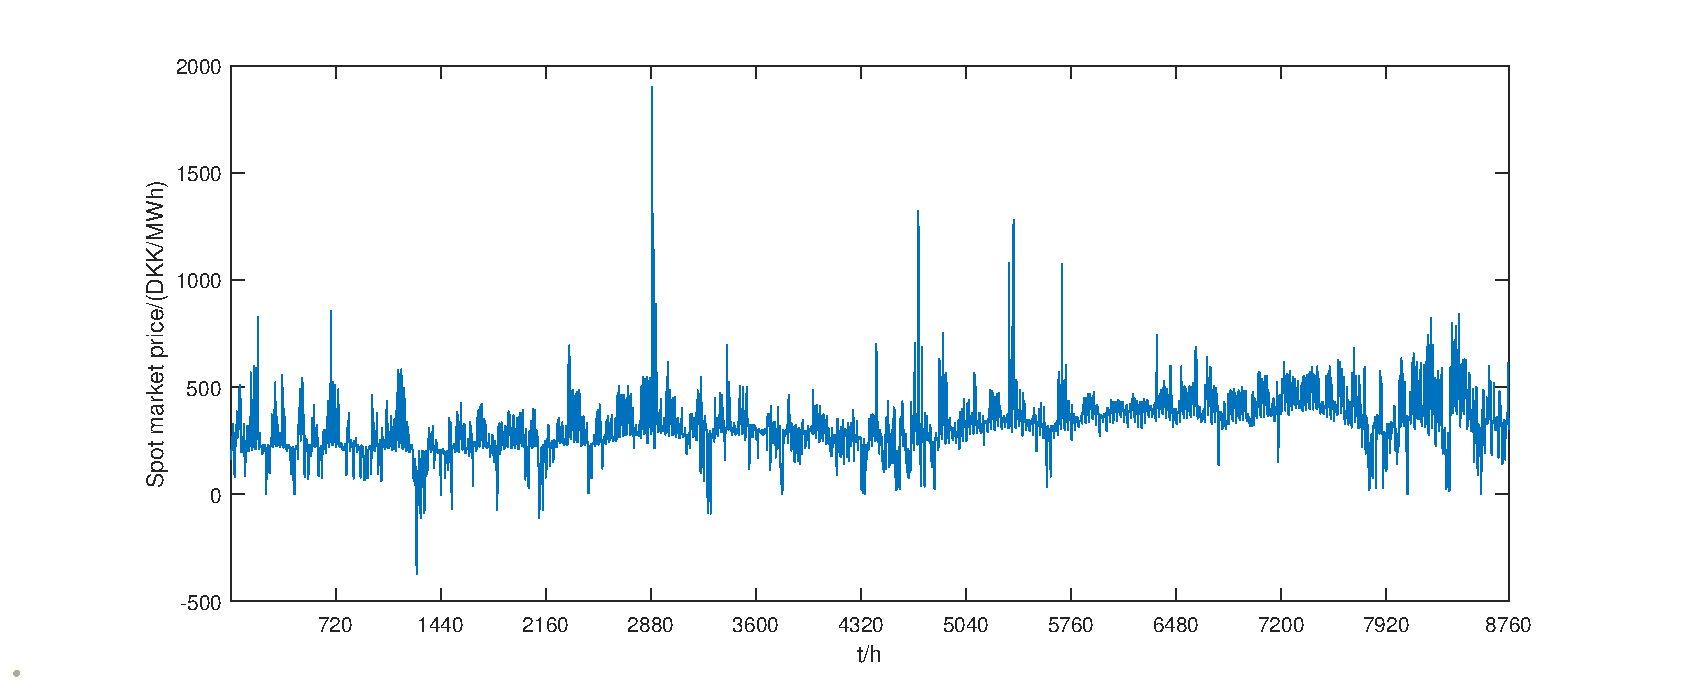
\includegraphics[width=0.5\textwidth]{figures/elspot.eps}
    \caption{The spot market prices for a year}
    \label{fig:elspot}
\end{figure}

\subsection{Reference wind farm}
\begin {table}[h]
\small
\centering
 \begin{threeparttable}
 \caption{Economical analysis parameters}
 \vspace{5pt}
 \begin{tabular}{lcc}
\hline
\textbf{Parameter}& \textbf{Values}&\textbf{References}\\ 
\hline
Wind turbine lifetime&20 years & \\
Bi-directional inverter lifetime & 10 years& \cite{Hinkle2011}\\
RESS secondary service lifetime & 7 years & \cite{Jiao2018BusinessBatteries, Ambrose2014DrivingBatteries}\\
Discount rate $d_r$& 5\% & \\
O\&M ratio $r_{O\&M}$ for RESS and inverter & 1\%/year & \cite{Zhang2017ComparativeOperation}  \\
Bi-directional inverter price/kWh  & 1000 DKK&\\
Brand new EV battery price/kWh & 1787 DKK & \cite{BNEF2017} \\
Brand new EV battery stack capacity & 24kWh&\\
SoH\tnote{*} of retired EV batteries&80\% & \cite{Abdel-monemLithium-ionKeywords,Zhai2017ModelingMarket,Hu2018OptimizationLoads}\\
Maximum charging/discharging rate & By inverter& \\
Charging/discharging efficiency & 95\% & \cite{Abdel-monemLithium-ionKeywords}\\
Inverter efficiency & 98\% & \cite{Wolfs2015}\\
Maximum SoC&80\%&\\
Minimum SoC&20\%&\\
Initial(End-of-day) SoC(case 1)&20\%&\\
Initial(End-of-day) SoC(case 2)&35\%&\\
\hline
\end{tabular}
        \label{tab:cba}
\begin{tablenotes}
        \footnotesize
        \item[*] State of health, the ratio between usable capacity and nominal capacity.
        \end{tablenotes}
    \end{threeparttable}
\end {table}
The wind farm near the Danish island Sprogoe consist of seven Vestas V90-3 MW wind turbines. Using WindPro and the mesoscale wind data from ERA5, the hourly electricity production from each of the wind farm has been calculated between November 1, 2017 and October 31, 2018. The expected lifetime of an offshore wind farm is 20-25 years \cite{Hou2017OffshoreOptimization}.  The location of Sprogoe is in the middle of the Great Belt of Denmark, which had 11,357,037 personal vehicles passing by in 2018 \cite{Storebaet}, making it an ideal position for a nearby EV charging station.
\begin{figure}[h]
    \centering
    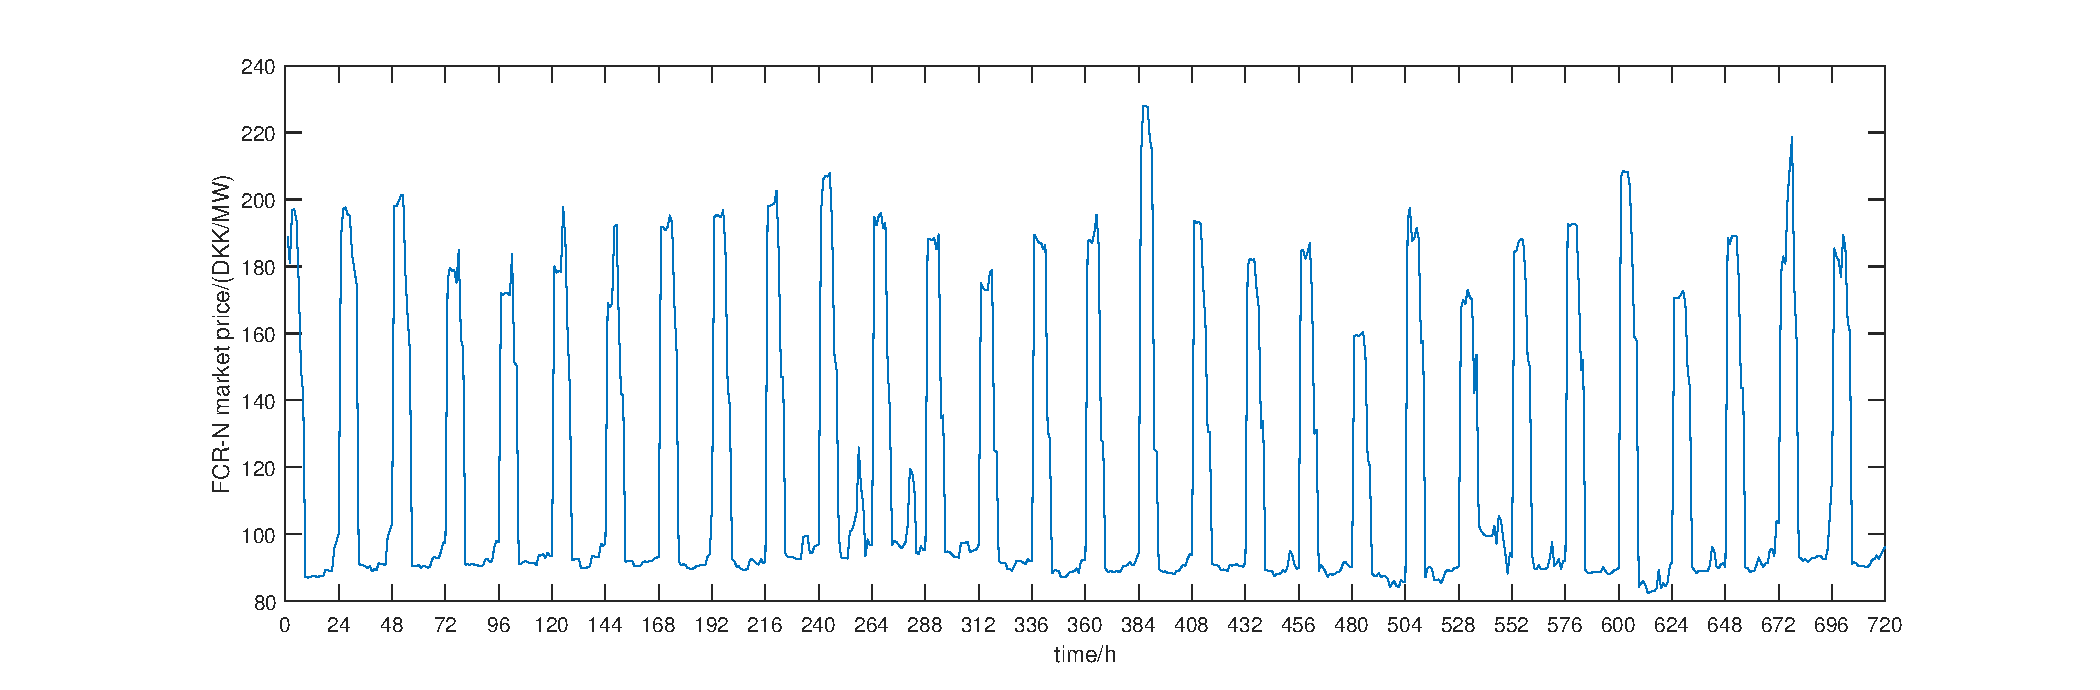
\includegraphics[width=0.5\textwidth]{figures/FCRN.eps}
    \caption{The FCR-N market prices from 31/12/2017 to 28/1/2018}
    \label{fig:FCRN}
\end{figure}

\subsection{Retired EV battery}
Nissan Leaf is the bestselling EV model in Norway (over 50,000 in total) \cite{Elbilstatistikk}, and had a market share of 50\% of the Danish EV market in 2018 \cite{Nissan}.  The first 24kWh Leaf model entered the Danish market around 2011 and  was  warrantied  for  8  year’s  life  span  or  100,000  mileage \cite{Nissan1},  which  makes  today  around the  peak  of  retirement for this model. The retired EV  batteries  are  connected  in  stack  to work as a RESS for the hybrid system, the capacity of which (i.e.  number of connected batteries) and the installed inverter capacity are optimized to achieve maximum profit. The specification of the RESS and inverter can be found in Table \ref{tab:cba}. Two scenarios concerning the price of retired EV battery are considered. In the optimistic scenario, the price is 15\% of its brand new model price. While in the pessimistic scenario, the price is considered as 30\% of that.

\begin{figure}[h]
    \centering
    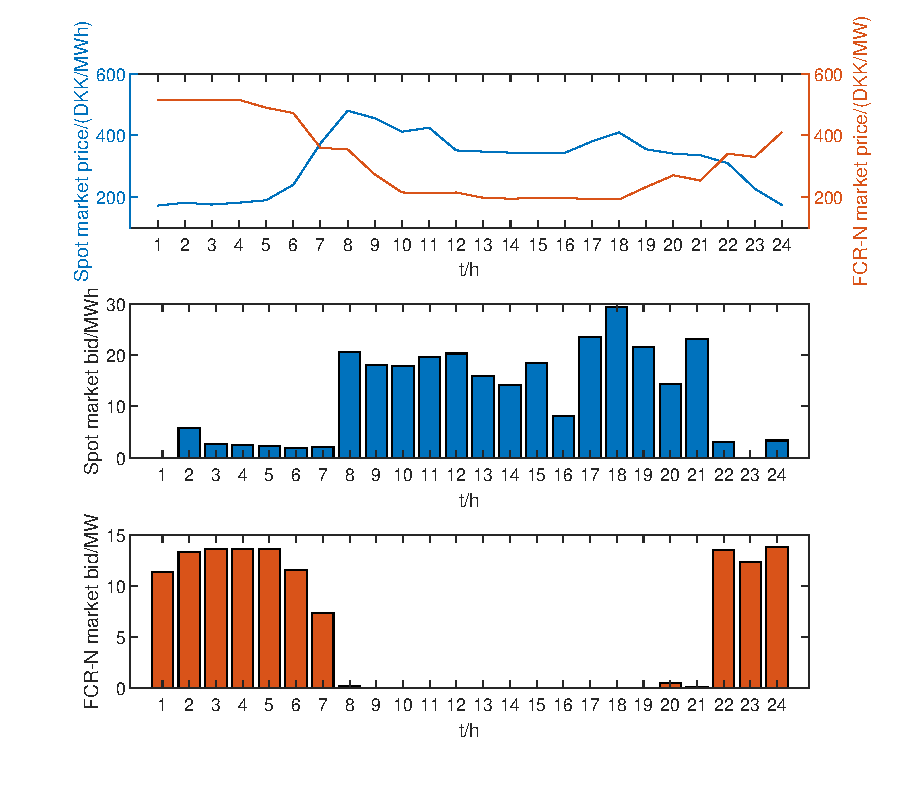
\includegraphics[width=0.5\textwidth]{figures/bids.eps}
    \caption{Bids in the spot market and the reserve market in the optimistic scenario}
    \label{fig:bids}
\end{figure}

\subsection{Optimization results}
In the implementation of the stochastic programming framework, to account the uncertainties in the model, a large number of scenarios (1000 in this case) have been generated with MCS and RWM. A SBM is afterwards applied to reduce the generated scenarios to 20 remained, in line with \cite{Ahmadi2016}. A sensitivity analysis is provided in section \ref{sec:sensitivity} to investigate the influence of the amount of the remained scenarios on the final results. 

\begin{table*}[h]
    \caption{Optimization results}
     \vspace{5pt}
    \centering
    \begin{threeparttable}
    \begin{tabular}{lccccccc}
    \hline
        \textbf{Scenario}\tnote{1}& \textbf{Battery Number} & \textbf{Inverter Size} & \textbf{Yearly Revenue } &\textbf{ NPV-C}&\textbf{ \text{NPV-P}} &\textbf{RoI}\tnote{2}&\textbf{PBY}\tnote{3}\\
        \hline
        Base case &  & & 18.20 M\tnote{4}&  &  &  &  \\
         \hline
         Case 1(optimistic) & 0&0&  18.20 M & 0 &0 &&\\
    
         Case 1(pessimistic)& 0&0&  18.20 M &0  &0 &&\\
         \hline
         Case 2(optimistic) & 1615 & 13.88 MW&  24.59 M  & 48.60 M&35.04 M &72.10\%&4.27\\
          Case 2(pessimistic) &895&9.41MW& 22.75 M &43.44 M&16.10 M&37.07\%&5.34\\
         \hline
    \end{tabular}        \label{tab:results}
     \begin{tablenotes}
        \footnotesize
        \item[1] The optimization span is a year with the daily boundary conditions and a time resolution of an hour.
        \item[2] Return on Investment, $RoI = \frac{\text{NPV-B}}{\text{NPV-C}}$
        \item[3] Payback Year: time when the net present benefit equals investment.
        \item[4] Million DKK.
      \end{tablenotes}
    \end{threeparttable}
\end{table*}

In this study, two cases with both the optimistic and pessimistic scenarios are examined. As in Table \ref{tab:results}, the wind farm cannot recover its investment introducing a RESS and an inverter even in the optimistic scenario in case 1, where the wind farm only forwards bids in the spot market, which is primarily due to the high inverter and battery prices considering the spot market prices are highly variable as in Fig. \ref{fig:elspot}, with a daily average standard deviation of 66.8 DKK/MWh .

While in case 2 under the optimistic scenario, the wind farm would like to install 1615 single retired batteries to form a RESS with a disposable capacity of 30.0 MWh due to battery degradation and an inverter of 13.9 MW, which would lead to an annual revenue increase of 6.4 MDKK. As the result indicates, the wind farm will recover its initial investment after 4.3 years, with a overall return on investment (RoI) of 72.1\% over 20 years. In the pessimistic scenario, the wind farm would purchase a much smaller system with 895 single retired batteries and a 9.4 MW inverter. Even though with the yearly revenue dropping down by 1.8 MDKK, payback year increasing by 1.1 year, and almost halved RoI, the hybrid system is still on a financially competitive level. 
\begin{figure}[h]
    \centering
    \includegraphics[width = 0.5\textwidth,height =0.25\textwidth ]{figures/reserveActi.eps}
    \caption{Bids in the FCR-N market and reserve service activation in the optimistic scenario}
    \label{fig:reserveActi}
\end{figure}

The bids forwarded in both the spot market and the FCR-N market are taken as scenario-weighted mean values. In a typical day the spot market prices cross the FCR-N market prices, which is usually the case as shown in Fig. \ref{fig:FCRN} where the FCR-N market prices show a strong regularity of starting at a high level, dropping down drastically and bouncing back a little within a day. As a result, the bids made in the FCR-N market shows a similar pattern as in Fig. \ref{fig:bids}, being on a high level during the start as well as end of the day and around 0 in the middle of the day, when most of the wind power is transmitted to the spot market. Despite of this, the wind farm still receives a NPV of profit increase of 35.0 MDKK over 20 years in the optimistic scenario, verifying the high profitablity of participating the FCR-N market.
\begin{figure}[h]
    \centering
    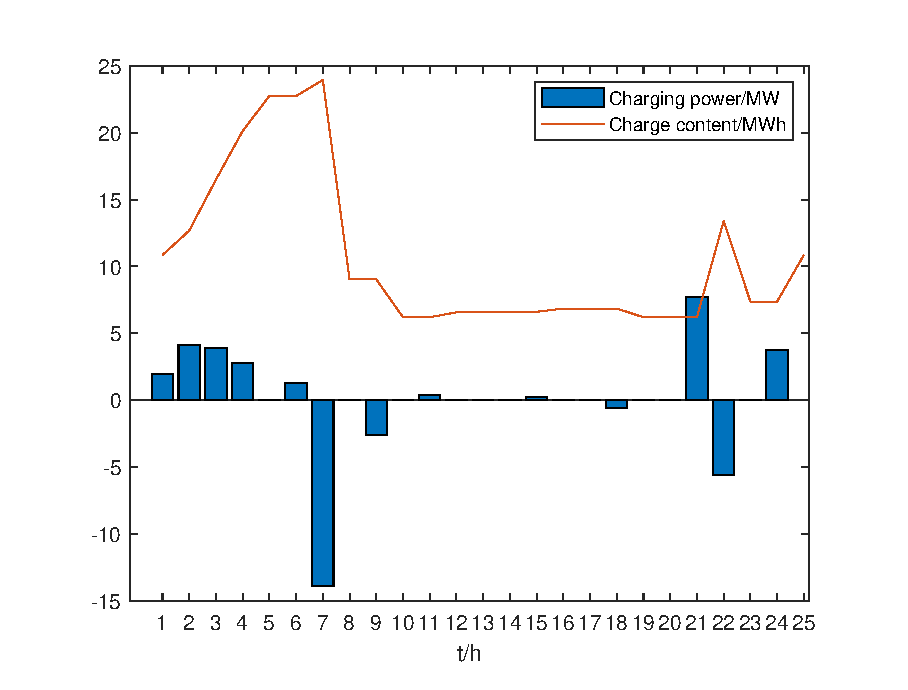
\includegraphics[width = 0.5\textwidth,height =0.25\textwidth]{figures/soc.eps}
    \caption{Energy content and charge/discharge in the optimistic scenario}
    \label{fig:socFig}
\end{figure}

\begin{figure}[h]
    \centering
    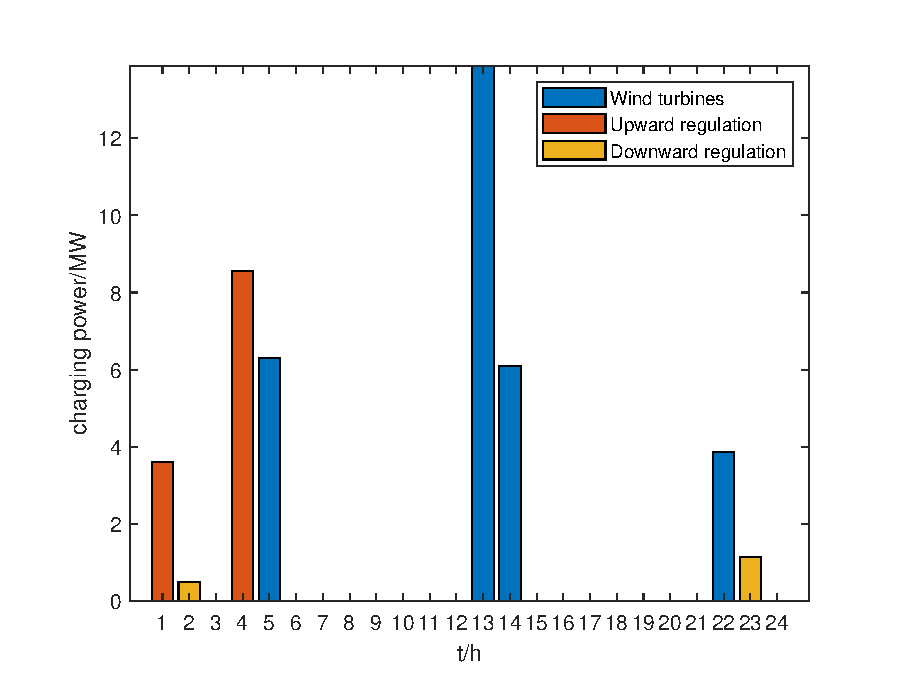
\includegraphics[width = 0.5\textwidth,height =0.25\textwidth]{figures/charge.eps}
    \caption{Charging power source in the optimistic scenario}
    \label{fig:charge}
\end{figure}

In Fig. \ref{fig:reserveActi}, the reserve service activation is depicted in two different directions, indicating upward regulation and downward regulation for a certain scenario respectively. In the hours (3rd, 5th 6th, 22nd and 24th), the reserve services are not activated, though bids are forwarded to the market, which incurs loss in the revenue since the FCR-N market prices in the 22nd hour (334 DKK/MW) are lower than that of the spot market (344 DKK/MWh). However, this does not indicate the model is defected, since assuming the wind farm can precisely predict the frequency regulation directions a day before to make decisions as dictated in the model with binary variables is far too idealistic. The assumption that the wind farm always bids in the FCR-N market as long as the price is over 80\% of the spot market price is a compromise between situations when service is upwards activated so extra electricity can be reserved thus with extra revenues and cases when there is no activation so with economic losses, which makes the model more down to earth and the profit result more reliable.

In a typical scenario, the electricity flow profile of the RESS is as Fig. \ref{fig:socFig}, where the RESS discharges with a high rate at some moment in order to level off the charged energy within a day to satisfy the boundary conditions, which results in a high-capacity inverter. The charging profile is further divided in Fig. \ref{fig:charge} indicating that the wind power and the reserve service activation by upward regulations are the major sources of battery charging power.

\subsection{Sensitivity analysis}\label{sec:sensitivity}
\begin{table*}[h!]
    \centering
     \caption{Sensitivity analysis results}
    \begin{tabular}{ccccc}
    \hline
        \textbf{Remained scenarios} & \textbf{Battery Number} &\textbf{Inverter size}
        &\textbf{NPV-P}
        & \textbf{Normalized computation time}\\
         \hline
         Non-stochastic & 1622 & 12.99 MW & 30.96 MDKK & 0.015\\
         5&1640 & 13.83 MW& 34.98 MDKK & 0.09\\
         10  & 1615&13.89 MW& 35.08 MDKK & 0.25\\
         20&1615 &13.88 MW&35.04 MDKK&1 \\
         \hline
    \end{tabular}
    \label{tab:sensitivity}
\end{table*}
In this section, a sensitivity analysis is employed to investigate the influence on the planning and financial results of the remained scenarios number after applying the SBM. We specifically focus on case 2 for the optimistic scenario. The case when the stochastic framework is not applied is also included, in which the markets prices, wind power and regulating statuses are all historic data. The solving time is normalized based on the case where 20 scenarios remain after the scenario reduction technique. The equipment sizes and the normalized solving times are shown in Table \ref{tab:sensitivity}.

From the sensitivity analysis results, following conclusions can be obtained: 1) The computation time is highly influenced by the number of remained scenarios. When the scenario number doubles, the solving process takes 3-4 times longer. 2) The planning results stabilise at larger number of scenarios. In this case, 10 remained scenarios give almost the same results as 20 scenarios. 3) In this case, 10 remained scenarios gives the best performance in terms of optimization accuracy and computation time.


\section{Conclusion}
In this study, a hybrid wind turbine-retired battery storage system is proposed to participate both the spot market and the FCR-N market to increase the wind farm owner's profit. The uncertainties are modelled with a scenario-based stochastic programming method. The scenarios are generated with MCS and RWM. Afterwards, they are applied to SBM to be reduced to enhance the computational efficiency. The hybrid system are investigated in two cases. In the first case, the wind farm participate in the spot market only. While in the second case, the wind farm also forwards bids in the FCR-N market. Two scenarios (optimistic/pessimistic) are raised in terms of the price of retired EV batteries to examine its influence on the planning. A sensitivity analysis is performed at last to provide insights regarding the influence of remained number of scenarios on the optimization results.

The optimization results show that by integrating the retired EV batteries and forwarding bids in the FCR-N market, the system can increase the net present value of profit by 35.0 MDKK in the optimistic scenario and 16.1 MDKK in the pessimistic scenario. Compare case 1 with case 2, participating FCR-N market is the major reason of the increased profit when the wind farm integrates retired EV batteries. The sensitivity analysis concludes that 10 remained scenarios would have the best performance regarding optimziation accuracy and computation efficiency. Considering the fact that brand new EV battery price was dropping dramatically over the years (73\% drop from 2010 - 2016) \cite{BNEF2017} and is expected to be further decreased down to 109 \$/kWh in 2025 and 73 \$/kWh in 2030 \cite{BNEF2017}, the proposed system is highly financially favourable and provides an alternative to repurpose the retired EV batteries.


%% The Appendices part is started with the command \appendix;
%% appendix sections are then done as normal sections
%% \appendix

%% \section{}
%% \label{}


\section*{References}
\bibliographystyle{elsarticle-num} 
\bibliography{reference}



\end{document}

\endinput

